\documentclass[../main_proj3.tex]{subfiles}

\graphicspath{{\subfix{Figures/}}}

\begin{document}

\section{Methods and theory}\label{sec:methods_and_theory}

\subsection{The Penning trap}

- introduction on the penning trap and illustration
\begin{figure}[h!]
    \centering
    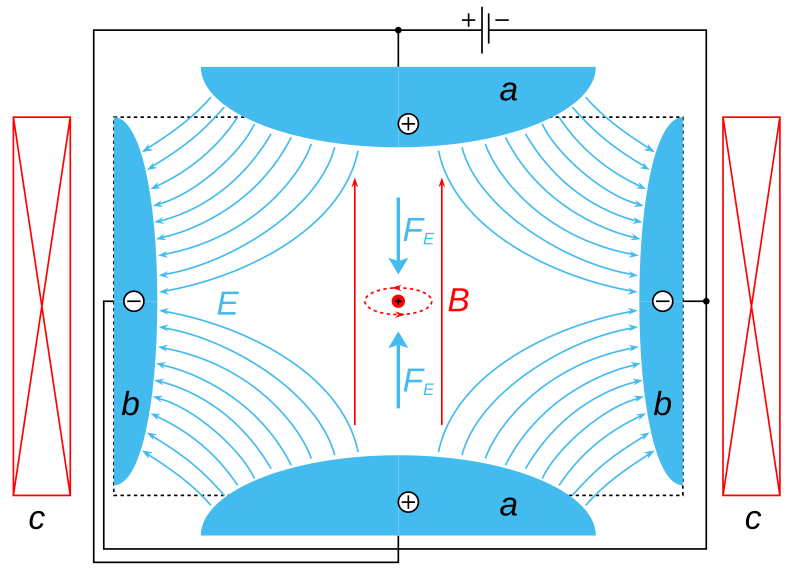
\includegraphics[width=0.9\linewidth]{Project 3/figures/Penning_Trap.png}
    \caption{Illustration from Wikipedia.org \cite{PenningTrapIllustration}.}
    \label{fig:Penning_trap}
\end{figure}

- defining all parts of the trap and so on.


The electric field $\mathbf{E}$ is related to the electric potential $V$ by 
\begin{equation}
\label{eq:electric_field-electric_potential}
\mathbf{E} = - \nabla V \quad, 
\end{equation}

where we in this study consider an ideal Penning trap where the electric potential is given by 

\begin{equation}
\label{eq:electric_potential}
V(x,y,z) = \frac{V_0}{2d^{2}} (2z^{2} - x^{2} - y^{2}) \quad.
\end{equation}

In equation \eqref{eq:electric_potential} $V_0$ is the potential applied to electrodes of the Penning trap (the end caps and the ring indicated by (a) and (b) in Figure \ref{fig:Penning_trap}). Lastly the characteristic dimension $d=\sqrt{z_0^{2}+r_0^{2}/2}$ represents the length scale between electrodes defined by the distance from the center to the end caps $z_0$ and to the ring $r_0$. 

Solving equation \eqref{eq:electric_field-electric_potential} for equation \eqref{eq:electric_potential} yields

\begin{equation}
\label{eq:solved_electric_field}
\begin{split}
\mathbf{E} & = - \nabla V \quad \\
& = - \frac{V_0}{2d^{2}} \nabla \left[2z^{2}-x^{2}-y^{2}\right] \\
& = - \frac{V_0}{2d^{2}} 
\bigl\langle 
2x, 2y, -4z
\bigr\rangle \quad ,
\end{split}
\end{equation}

which implies that a charge particle $q$ will be trapped axially (the $z$ direction) due to ... . To trap radially the Penning trap imposes a homogeneous magnetic field 
\begin{equation}
\label{eq:magnetic_field}
\mathbf{B} = \bigl\langle 
0, 0, B_0
\bigr\rangle \quad ,
\end{equation}

where $B_0 > 0$ is the magnitude of the field strength. Modelling a charged particle as a point charge, it will set up an electric field in position $\mathbf{r}$ that is proportional to the particle charge $q$ and the distance from the particle and an arbitary position $\mathbf{r}$. If the Penning trap host's multiple point charges $\{q_1, \dots, q_n\}$ with positions $\{\mathbf{r}_1, \dots, \mathbf{r}_n\}$ they will set up an electric field given by the superposition of the individual fields setup by particle $j$. The resulting field is given by 
\begin{equation}
\label{eq:electric_field_particles}
\mathbf{E} = k_e \sum\limits_{j=1}^n \frac{\mathbf{r}-\mathbf{r}_j}{|\mathbf{r}-\mathbf{r}_j|^{3}} \quad.
\end{equation}


\subsection{The equations of motion}

For the Penning trap the time evolution of a particle is given by Newton's second law 
\begin{equation}
\label{eq:newtons_second_law_Penning_trap}
m \mathbf{\ddot{r}}  = \sum_i \mathbf{F_i} \quad ,
\end{equation}
where $\mathbf{\ddot{r}}:=\frac{d^{2}\mathbf{r}}{dt^{2}}$ is the acceleration of the particle given its position in space $\mathbf{r}$ and $\mathbf{F}$ is the Lorentz force

\begin{equation}
    \label{eq:Lorentz-force}
    \mathbf{F} = q\mathbf{E} + q \mathbf{v} \times \mathbf{B} \quad .
\end{equation}

Here $\mathbf{E}$ is given by equations \eqref{eq:solved_electric_field} and \eqref{eq:electric_field_particles} however for this derivation we assume the number of particles to be one so we leav out the interactions. The cross product is solved as 

\begin{equation}
\label{eq:cross_product}
\begin{split}
q \mathbf{v} \times \mathbf{B} & =  q \bigl\langle 
\dot{x}, \dot{y}, \dot{z}
\bigr\rangle \times \bigl\langle 
0, 0, B_0
\bigr\rangle \\
&= qB_0 \bigl\langle
\dot{y}, -\dot{x}, 0
\bigr\rangle 
\end{split} \quad .
\end{equation}

Substituting equation \eqref{eq:solved_electric_field} \eqref{eq:cross_product} and \eqref{eq:Lorentz-force} into equation \eqref{eq:newtons_second_law_Penning_trap} yields the equation 

\begin{equation*}
m \mathbf{\ddot{r}} = - q \frac{V_0}{2d^{2}} 
\bigl\langle 
2x, 2y, -4z
\bigr\rangle + qB_0 \bigl\langle
\dot{y}, -\dot{x}, 0
\bigr\rangle  \quad,
\end{equation*}

which for $\hat{e}_x$ becomes

\begin{equation}
\label{eq:eq_of_motion_x}
\begin{split}
m \ddot{x} & = q(- \frac{V_0}{2d^{2}}2x + B_0 \dot{y}) \\
\ddot{x}  &= \omega_0 \dot{y} + \frac{1}{2} \omega_z^{2} x
\end{split}
\end{equation}

by defining $\omega_0 :=\frac{qB_0}{m}$ and $\omega_z^{2} := \frac{2qV_0}{md^{2}}$. Similarly for $\hat e_y$ the equation becomes 
\begin{equation}
\label{eq:eq_of_motion_y}
\ddot{y}  = \omega_0 \dot{x} + \frac{1}{2} \omega_z^{2} y \quad ,
\end{equation}

while for $\hat e_z$ we have $qB_0 \cdot 0$ so the expression simplifies to 

\begin{equation}
\label{eq:eq_of_motion_z}
\ddot z = - \omega_z^{2} z \quad .
\end{equation}

From these equations it is apperent that ... enhetsvektorene styrt av elektrisk og magnetisk potensial. 

The system of equations \eqref{eq:eq_of_motion_x}, \label{eq:eq_of_motion_y} and \label{eq:eq_of_motion_z} consists of three equations where equation \eqref{eq:eq_of_motion_x} and \eqref{eq:eq_of_motion_y} are coupled. To find a general solution, start by rewriting these in terms of one differential equation by introducing a complex function $f(t)=x(t) + iy(t)$. Since $i= \sqrt{-1}$ is a \textit{const.} the first- and second-order derivatives become (using the dot notation and omitting the dependency towards $t$) $\dot f = \dot x + i \dot y$ and $\ddot f = \ddot x + i \ddot y$, respectively. By substituting equations \eqref{eq:eq_of_motion_x} and \eqref{eq:eq_of_motion_y}, solved for $x$ and $y$ respectively, into the complex function the pair can be compressed into one equation 

\begin{equation}
\label{eq:eq_of_motion_f}
\begin{split}
    f & = x + iy \\
    f & = (\ddot{x} - \omega_0 \dot{y}) \frac{2}{\omega_z^{2}} + i (\ddot{y} - \omega_0 \dot{x}) \frac{2}{\omega_z^{2}} \\
    \frac{1}{2} \omega_z^{2} f & = \ddot{x} + i\ddot{y} - \omega_0 \dot{y} - i \mega_0 \dot{x} \\
    \ddot{f} - \frac{1}{2} \omega_z^{2} f &= - \omega_0 ( \dot{y} +i \dot{x}) \\
    \ddot{f} & = \frac{1}{2} \omega_z^{2} f - i \omega_0 \dot{f}
\end{split}
\end{equation}

where we have identified that $\dot{y} +i \dot{x}$ in line four is equal to the imaginary unit times the complex conjugate of $f$; $i\dot{f}^* = i(\dot{x} - i\dot{y}) = \dot{y} + i \dot{x}$. Since $\dot{f}$ is a scalar and not a vector, it represents the \textit{speed} and not the \textit{velocity}, that consequence is that it is a real valued function of time and thus $\dot{f}^* = \dot{f}$. This equation describes the particle movement in the radial plane (xy-plane).

The general solution to \eqref{eq:eq_of_motion_f} is 
\begin{equation}
\label{eq:general_solution-eq_of_motion_f}
    f(t) = A_+ e^{-i(\omega_+ t + \phi_+)} + A_- e^{-i(\omega_- t + \phi_-)} \quad ,
\end{equation}

where $\phi_+$ and $\phi_-$ are constant phases, the amplitudes $A_+$ and $A_-$ are positive, and 
$$
\omega_\pm = \frac{\omega_0 \pm \sqrt{\omega_0^2 - 2\omega_z^2}}{2} \quad.
$$
The physical coordinates are then found as $x(t) = \text{Re}\big[f(t)\big]$ and $y(t) = \text{Im} \big[f(t)\big]$.

To obtain a bounded solution for the movement in the radial plane, we require $|f(t)| < \infty$ as $t\to \infty$. This implies that constraining the frequencies $\omega_\pm$ to be real as complex roots will make the exponent of the exponentials in equation \eqref{eq:general_solution-eq_of_motion_f} positive, which will lead to a violation of the constraint in $f(t)$. To ensure real roots, we need 

\begin{equation}
\label{eq:frequency_constraint}
\begin{split}
    \omega_0^{2} - 2\omega_z^{2} &\geq 0 \\ 
    \frac{q^{2}B_0^{2}}{m^{2}} - 2\left(\frac{2qV_0}{md^{2}}\right) & \geq 0 \\
    \frac{q^{2}B_0^{2}}{m^{2}} & \geq 4 \frac{qV_0}{md^{2}} \\
    \frac{B_0^{2}d^{2}}{V_0} &\geq \frac{m}{q} \quad ,
\end{split}
\end{equation}

which means that the ratio between particle mass and charge must be less than or equal to the ratio between the squared product of the magnetic field strength and the characteristic length and the electric field strength. Physically, this implies that a stronger magnetic field is required if the electric field strength is increased. It also implies that increasing $B_0$ will make it easier to meet the stability requirement and that decreasing $d$ will reduce the stability given fixed values of $B_0$ and $V_0$.  

It is also important to find the bounds of the particle's distance from the origin in the radial plane. To find the upper bound $R_+$ we need to maximize the exponential parts of equation \eqref{eq:general_solution-eq_of_motion_f} 

\subsection{Benchmark solution}

To benchmark the numerical modelling of this initial value problem we will derive a specific analytical solution for a single particle $p$, defined in the project description \cite{prosjekttbeskrivelse3}. The particle $p$ holds a charge $q$ and mass $m$ while it is in the Penning trap. Initially it occupies the position 
$\mathbf{r_0} = \bigl\langle x(0), y(0), z(0) \bigr\rangle = \bigl\langle x_0, 0, z_0 \rangle$ and has the initial velocity $\mathbf{v}_0 = \bigl\langle 
\dot{x}(0), \dot{y}(0), \dot{z}(0)
\bigr\rangle = \bigl\langle 
0, v_0, 0 \bigr\rangle$. Further the specific solution to equation \eqref{eq:eq_of_motion_z} given the initial position $z_0$ is 
\begin{equation}
\label{eq:specific_solution-eq_of_motion_z}
z(t) = z_0 cos(\omega_z t) \quad.
\end{equation}

Further, the \textit{specific} solution to equation \eqref{eq:general_solution-eq_of_motion_f} is given by the amplitudes and phases 
\begin{equation*}
\begin{split}
    A_+ & = \frac{v_0 + \omega_-x_0}{\omega_- - \omega_+} \quad ,\\
    A_- & = - \frac{v_0 + \omega_+ x_0}{\omega_- - \omega_+} \quad , \\
    \phi_+ &= 0\quad , \\
    \phi_- & = 0    \quad.
\end{split}
\end{equation*}

We will use singly-charge calcium ions (Ca$^{+}$) as our particles for this project and the units will be; the micrometre ($\textrm{\mu m}$) for length, microseconds ($\textrm{\mu s}$) for time, the atomic mass unit ($\textrm{u}$) for mass and the  elementary charge ($\textrm{e}$) for charge.  This is done to reduce round-off errors that occur when working with very small numbers e.g. when considering the particle mass $m_{Ca^{+}} = 40.078 ~\mathrm{u}$ which is on the order of $10^{1}$ instead of $\mathcal{O}(m_{Ca} (kg)) = 10^{-26}$ (using $m_{Ca^{+}}\approx m_{Ca}$ since the mass of the added electron is negligible $\mathcal{O}(m_{e}) = 10^{-31} \mathrm{kg} << \mathcal{O}(m_{Ca})$).

In these units, the Coulomb constant is $k_e = 1.38935333 \times 10^5 \, \frac{\textrm{u} \, (\textrm{\mu m})^3}{(\textrm{\mu s})^2 \, \textrm{e}^2}$ and the derived SI units for the magnetic field strength (Tesla, $\textrm{T}$) and the electric potential (Volt, $\textrm{V}$) become $\mathrm{T} = 9.64852558 \times 10^1 \, \frac{\mathrm{u}}{(\mathrm{\mu s}) \, \mathrm{e}}$ and $\mathrm{V} = 9.64852558 \times 10^7 \, \frac{\mathrm{u} \, (\mathrm{\mu m})^2}{(\mathrm{\mu s})^2 \, \mathrm{e}}$.

Further, for a benchmark solution we set the magnetic field strength to $B_0 = 1.00\,\mathrm{T} \simeq 9.65 \times 10^1 \, \frac{\mathrm{u}}{(\mathrm{\mu s}) \, \mathrm{e}}$, the applied potential to $V_0 = 25.0\,\mathrm{mV} \simeq 2.41 \times 10^6 \, \frac{\mathrm{u} \, (\mathrm{\mu m})^2}{(\mathrm{\mu s})^2 \, \mathrm{e}}$ and the Penning trap characteristic dimension to $d = 500\,\mathrm{\mu m}$. Throughout the derived equations $V_0$ and $d$ only appear as the ratio $\frac{V_0}{d^{2}} = \frac{25 \mathrm{mV}}{500 \mathrm{\mu m}} = 9.65  \frac{\mathrm{u}}{(\mathrm{\mu s})^2 \, \mathrm{e}}$.


Considering the initial values $x_0 = z_0 = 20 \mathrm{\mu m}$ and $v_0 = 25 \mathrm{\mu m \mu s^{-1}}$ the solution, simulating a single Ca$^{+}$ ion from $t=0\mathrm{\mu s}$ to $t= 50 \mathrm{\mu s}$ becomes:

\begin{equation*}
\begin{split}
    
\end{split}
\end{equation*}

\subsection{dummy method's}

\textit{The main purpose of the ``Methods'' (or ``Theory'', or ``Algorithms'') section is to provide the reader with the necessary background knowledge to understand the work you will present.\footnote{Note that to get correct quotation marks in LaTeX, you cannot simply use the quotation mark symbol on your keyboard. Check the \texttt{.tex} file for this document to see the correct approach.} It should in general be sufficiently detailed for the reader to understand and reproduce what you have done. However, sometimes it can be a good idea to relegate the discussion of some technical topic to an appendix, to avoid too long discussions of what might be a a fairly minor or technical detail. You are of course free to divide this section into subsections, which we will do below.}

Let $f$ be a continuous and differentiable function, $f: [a,b] \to \mathbb{R}$. Say we want to integrate this function over the entire interval $[a,b]$. To this end, we employ the midpoint rule for integration, which is defined by the equation~\cite{Linear_Algebra_and_its_Applications}
%
\begin{equation}
\label{eq:midpoint_rule}
    I = \int_a^b f(x)\dd x \approx h\sum_{i=1}^{n} f(x_i).
\end{equation}
Here $n$ denotes a number of subintervals of the range $[a,b]$, each of length $h = (b-a)/n$, and $x_i$ is the midpoint of subinterval $i$, given by
\begin{equation}
   x_i = a + \left(i-\frac{1}{2}\right) h,
\end{equation}
for $i = 1, 2, \ldots, n$. This equation can be written out explicitly (although in this case it is a bit silly):
%
\begin{equation}
    \begin{split}
        \int_a^b f(x)\dd x & \approx h \sum_{i=1}^{n} f(x_i) \\
                                    \\
                                    & = h\left(f(x_1) + \cdots + f(x_{n})\right).
    \end{split}
\end{equation}
%
\textit{Note the following: We have provided a definition for every single variable that appears in the equations. Always do this --- it greatly improves the transparency and readability of your work! Once a variable is defined, you can reuse it throughout the rest of the report without stating its definition. (This of course assumes that you use consistent notation, so that a symbol does not suddenly change meaning in the middle of your report.)}

\textit{Also, note that we cited a source for our claim. There is no need to provide references for trivial or very well-known results, like Newton's second law, but you should cite material that is vital for your report.}

\textit{If you want to refer to a specific equation from elsewhere in your text, use the equation number, just like you would refer to a table or figure, but also include a parenthesis: ``In Equation \eqref{eq:midpoint_rule} we see that \ldots''. The best approach is to use the \texttt{eqref} command, which adds the parenthesis automatically.} 

\textit{Finally, please note the following two details on how to write equations: First, remember that equations are regarded as part of a sentence, meaning that you should follow the standard rules for punctuation. This typically means that your equations should be followed by a comma or a period. Second, make sure that you do not unintentionally include blank lines before or after the equation in your \texttt{.tex} file. LaTeX interprets blank lines as the beginning of a new paragraph, and will therefore indent the text after the equation. If you prefer having a bit of ``air'' in your LaTeX document, use an empty comment line.}

To test our integration algorithm we will use it to integrate the polynomial $f(x) = x^3$ over the interval $[a,b] = [0,1]$. This is a suitable test case, since the integral has a known analytical solution,
\begin{equation}
    \int_0^1 x^3 \dd x = \frac{1}{4}.
\end{equation}
In assessing the performance of our approach we will consider the relative error $\epsilon$, defined as
\begin{equation}
    \epsilon = \abs{ \frac{I - I_{\text{approx}}}{I} },
\end{equation}
where $I$ denotes the exact integral and $I_\text{approx}$ denotes the approximation obtained with our implementation of the midpoint rule algorithm.

% -------------------------------------------
\subsection*{The algorithm}
%
The algorithm for the midpoint rule is summarized in Algorithm~\ref{algo:midpointrule}. The basic idea behind the algorithm is to divide the integration range into to $n$ small subintervals of length $h$, and on each such subinterval approximate the function $f(x)$ by a constant function. The value for this constant function is taken to be the value of $f(x)$ evaluated at the midpoint of the given subinterval --- hence the name of the method.
%
\begin{figure}
% NOTE: We only need \begin{figure} ... \end{figure} here because of a compatability issue between the 'revtex4-1' document class and the 'algorithm' environment.
    \begin{algorithm}[H]
    \caption{Midpoint rule for integration}
    \label{algo:midpointrule}
        \begin{algorithmic}
            \Procedure{Midpoint rule}{$f, a, b, n$}
            \State $I \leftarrow 0$        \Comment{Initialize the integral variable}
            \State $h \leftarrow (b-a)/n$  \Comment{Compute the interval length}
            \For{$i = 1, 2, \ldots, n$}
            \State $x \leftarrow a + (i-1/2)h$  \Comment{Assign $x$ to the midpoint}  %This means x is assigned the value x + ih/2.
            \State $I \leftarrow I + f(x)$  \Comment{Add contribution to integral} %Assign I to I + f(x)
            \EndFor
            \State $I \leftarrow Ih$  \Comment{Finalize the computation}
            \EndProcedure
        \end{algorithmic}
    \end{algorithm}
\end{figure}

\textit{As demonstrated in Algorithm~\ref{algo:midpointrule}, it is conventional to present algorithms in a way that is independent of any specific programming language. This ensures that it is the logic behind the algorithm that remains in focus, rather than the syntax of a particular programming language. In Algorithm~\ref{algo:midpointrule} we have also demonstrated a common notation: The right-to-left arrow ($\leftarrow$) means that we assign the value of everything on the right to the variable on the left. This is nothing but how the ``='' symbol functions in most programming languages, but the arrow notation makes it clear that we are in fact assigning a value, rather than stating that two things are equal.}

% -------------------------------------------
\subsection*{Tools}
%
\textit{This subsection is for informing the reader about the most important tools or software packages you have used, and what you have used them for. For instance, if you have used ChatGPT for anything, this subsection is where you should write about it.}

We used the Python library \texttt{matplotlib} \cite{Linear_Algebra_and_its_Applications} to produce all illustrations in this report. To parallelize our numerical integration code with \texttt{OpenMP}, we made use of examples taken from the tutorial in Ref.\ \cite{Linear_Algebra_and_its_Applications}.

\end{document}